\chapter{Invariante Gesetze, Vierervektoren und der Feldstärketensor}

Wir beginnen mit einem Gesetz, dem die Natur hätte folgen können, es aber nicht tut. Sein Scheitern zeigt uns, wie ein physikalisches Gesetz formuliert werden sollte. Derselbe Test führt zunächst von Koordinatenkomponenten zu gewöhnlichen Vektoren, dann von gewöhnlichen Vektoren zu Vierervektoren und schließlich von Vierervektoren zu Tensoren. Am Ende sind elektrische und magnetische Felder keine getrennten Objekte mehr: Zusammen belegen sie die sechs unabhängigen Komponenten eines antisymmetrischen Tensors.

Sofern nichts anderes angegeben ist, verwenden wir Einheiten, in denen \(c=1\) gilt, ordnen die Raumzeitkomponenten als \((1,2,3,0)=(x,y,z,t)\) an und verwenden die Metriksignatur \((-,-,-,+)\).

\section{Ein mögliches Gesetz mit der falschen Symmetrie}

Wir legen eine \(x\)- und eine \(y\)-Achse fest im Raum fest. Nun legen wir fest, dass zwei Teilchen wechselwirken, sobald ihre \(x\)-Koordinaten übereinstimmen. Die Wechselwirkung könnte ihre Bewegung umkehren oder sie in neue Richtungen treiben; auf die genaue Dynamik kommt es nicht an. Auslöser soll schlicht die Bedingung \begin{equation}
  x_1-x_2=0,
\end{equation} sein, wobei die Indizes Teilchen und nicht Koordinatenkomponenten bezeichnen. Diese Regel ist mathematisch widerspruchsfrei. Die Frage ist, was sie physikalisch unplausibel macht.

\begin{classroomqa}
\audiencequestion{Verletzt die Regel die Homogenität des Raums?}
\lecturerresponse{Nein. Eine Verschiebung des Ursprungs ändert beide Koordinaten um denselben Betrag und lässt \(x_1-x_2\) unverändert. Die Regel zeichnet keinen bestimmten Ort aus. Ihr Mangel liegt in der Isotropie: Sie zeichnet eine bestimmte Richtung aus.}
\end{classroomqa}

Drehen wir die Achsen um \(90^\circ\). Die bisherige \(x\)-Richtung heißt nun \(y\), sodass dieselben physikalischen Ereignisse durch die Gleichheit der \(y\)-Koordinaten beschrieben würden. Bei einem beliebigen Drehwinkel hinge die Bedingung von einer Linearkombination aus \(x\) und \(y\) ab. Die Form des Gesetzes hängt also davon ab, wie die Tafel ausgerichtet ist. Es ist translationsinvariant, aber nicht rotationsinvariant.

Physikalische Gesetze formulieren wir gewöhnlich in orthogonalen Koordinaten möglichst einfach. Man kann auch allgemeinere Koordinaten verwenden, doch dann werden die Metrik und die Formeln komplizierter. Innerhalb der Klasse orthogonaler kartesischer Bezugssysteme darf keine Ausrichtung ausgezeichnet sein.

Die Korrektur ist unmittelbar klar. In zwei Dimensionen müssen beide Koordinaten übereinstimmen, in drei Dimensionen alle drei: \begin{equation}
  x_1=x_2,
  \qquad y_1=y_2,
  \qquad z_1=z_2.
\end{equation} Dann können die Teilchen nur wechselwirken, wenn sie denselben Punkt erreichen, selbst wenn sie sich auf unterschiedlichen Geraden nähern.

\begin{classroomqa}
\audiencequestion{Müssen auch die \(z\)-Koordinaten und die Zeiten übereinstimmen?}
\lecturerresponse{Im dreidimensionalen Raum müssen auch die \(z\)-Koordinaten übereinstimmen. Die Zeit lassen wir vorerst außer Betracht; sobald die räumliche Argumentation abgeschlossen ist, beziehen wir sie wieder ein.}
\end{classroomqa}

Sei \(\boldsymbol r_a\) die Position des Teilchens \(a\). Die drei Komponentenbedingungen lassen sich zu einer Vektorgleichung zusammenfassen: \begin{equation}
  \boldsymbol r_1-\boldsymbol r_2=\boldsymbol 0.
\end{equation} Eine Komponente kann in einem gedrehten Bezugssystem verschwinden, in einem anderen jedoch nicht. Beim gesamten Vektor ist das anders: Sind in einem Bezugssystem alle Komponenten null, so sind sie es in jedem gedrehten Bezugssystem. Ebenso bleiben zwei Vektoren gleich, wenn sie in einem Bezugssystem gleich sind und beide transformiert werden.

\begin{figure}[H]\centering
\includegraphics[width=0.78\textwidth]{lecture_06_figure_01.png}\caption{Die drei Koordinatengleichheiten sorgen dafür, dass eine Kollision räumliches Zusammentreffen bedeutet und nicht das Zusammentreffen entlang einer ausgezeichneten Achse.}\lectureframe{00:09:00}\end{figure}

Darum sind Vektorgleichungen nützlich. Ihre Komponenten ändern sich, aber das Objekt transformiert sich als zusammenhängendes Ganzes. Ein Gesetz, das für das vollständige Objekt formuliert ist, kann seine Form bei einer Drehung der Koordinaten beibehalten.

\section{Zusammentreffen in der Raumzeit}

Ersetzen wir nun die vertikale räumliche Achse durch die Zeit. Ein Newtonsches Gesetz könnte besagen, dass zwei Bewegungsänderungen nur zu gleichen Zeiten stattfinden. In der Newtonschen Mechanik gilt die Gleichzeitigkeit für alle Inertialbeobachter gleichermaßen, daher ist ein solches Gesetz möglich. In der speziellen Relativitätstheorie zeichnet es jedoch ein bevorzugtes Bezugssystem aus. Ereignisse, die in einem Bezugssystem gleichzeitig sind, müssen es in einem anderen nicht sein.

Nur die Gleichheit der räumlichen Koordinaten zu verlangen, ist nicht besser. Eine Raumzeitverschiebung kann verschwindende räumliche Komponenten und zugleich eine von null verschiedene Zeitkomponente haben: \begin{equation}
  \Delta X^\mu=(0,0,0,\Delta t),
\end{equation} Außerdem mischt ein Boost \(\Delta t\) mit einer räumlichen Komponente. Die invariante lokale Aussage lautet, dass die beiden Bewegungsänderungen am selben Ereignis stattfinden. Eine einfache Kollision erfordert daher \begin{equation}
  X_1^\mu=X_2^\mu,
  \qquad\text{or}\qquad
  X_1^\mu-X_2^\mu=0.
\end{equation} Alle vier Koordinaten stimmen überein: Die Teilchen befinden sich zur selben Zeit am selben Ort.

Das Kollisionsbeispiel führt zu einer allgemeinen Regel für die Formulierung physikalischer Gesetze. Wir können alles auf eine Seite bringen und einen vollständigen Vierervektor gleich null setzen oder einen vollständigen Vierervektor einem anderen gleichsetzen. Gleichsetzungen einzelner, nicht zusammengehöriger Komponenten eines Vierervektors sind für sich genommen keine Lorentz-invarianten Aussagen.

\section{Boosts, Drehungen und Matrixschreibweise}

Ein Vierervektor ist ein Objekt, das sich so transformiert wie eine Raumzeitverschiebung. Um diese Definition nutzbar zu machen, betrachten wir zunächst noch einmal die Transformationen der Koordinaten selbst. Für einen Boost mit Geschwindigkeit \(v\) in \(x\)-Richtung gilt: \begin{align}
  x'&=\gamma(x-vt), & y'&=y, & z'&=z,
  & t'&=\gamma(t-vx),                                      \label{eq:l6-boost}
\end{align} Dabei ist \begin{equation}
  \gamma(v)=\frac{1}{\sqrt{1-v^2}}.
\end{equation}

\begin{classroomqa}
\audiencequestion{Wurde in diesen Formeln die Lichtgeschwindigkeit gleich eins gesetzt?}
\lecturerresponse{Ja. Um die Einheiten wieder einzusetzen, setzen wir \(X^0=ct\), ersetzen \(1-v^2\) durch \(1-v^2/c^2\) und ergänzen die entsprechenden Faktoren von \(c\) in den gemischten Raum--Zeit-Termen.}
\end{classroomqa}

Eine Drehung um die \(z\)-Achse mischt \(x\) und \(y\), während \(z\) und \(t\) unverändert bleiben: \begin{equation}
\begin{pmatrix}
  x'\\ y'\\ z'\\ t'
\end{pmatrix}
=
\begin{pmatrix}
  \cos\theta & \sin\theta & 0 & 0\\
  -\sin\theta & \cos\theta & 0 & 0\\
  0 & 0 & 1 & 0\\
  0 & 0 & 0 & 1
\end{pmatrix}
\begin{pmatrix}
  x\\ y\\ z\\ t
\end{pmatrix}.
\end{equation} Die Nullen sollte man ausdrücklich hinschreiben: So ist klar zu erkennen, welche Komponenten in die jeweilige transformierte Koordinate nicht eingehen. In derselben Reihenfolge lautet der Boost aus Gl.~\eqref{eq:l6-boost}: \begin{equation}
\begin{pmatrix}
  x'\\ y'\\ z'\\ t'
\end{pmatrix}
=
\begin{pmatrix}
  \gamma & 0 & 0 & -\gamma v\\
  0 & 1 & 0 & 0\\
  0 & 0 & 1 & 0\\
  -\gamma v & 0 & 0 & \gamma
\end{pmatrix}
\begin{pmatrix}
  x\\ y\\ z\\ t
\end{pmatrix}.
\end{equation}

Drehungen und Boosts lassen sich durch Matrixmultiplikation zusammensetzen. Um einen Boost in eine Richtung auszuführen, die nicht mit der ursprünglichen \(x\)-Achse übereinstimmt, kann man diese Richtung auf die \(x\)-Achse drehen, den Boost anwenden und anschließend nach Bedarf zurückdrehen. Produkte dieser elementaren Matrizen erzeugen allgemeinere Lorentz-Transformationen.

\begin{classroomqa}
\audiencequestion{Spielt es eine Rolle, ob man zuerst dreht und dann boostet oder zuerst boostet und dann dreht?}
\lecturerresponse{Ja. Nach dem ersten Schritt haben sich die Achsen geändert, auf die der zweite Schritt wirkt. Die beiden Matrixprodukte müssen daher nicht übereinstimmen; die Reihenfolge der Operationen ist also entscheidend.}
\end{classroomqa}

Alle diese linearen Transformationen lassen sich zusammenfassend schreiben als \begin{equation}
  X'^{\mu}=\Lambda^{\mu}{}_{\nu}X^{\nu}.                  \label{eq:l6-vector-transform}
\end{equation} Über den wiederholten Index \(\nu\) wird summiert, und zwar über \(1,2,3,0\). Das ist die gewöhnliche Zeile-mal-Spalte-Summe der Matrixmultiplikation, in Indexschreibweise ausgedrückt.

\begin{figure}[H]\centering
\includegraphics[width=0.78\textwidth]{lecture_06_figure_02.png}\caption{Die indizierte Lorentz-Transformation über ihrer Darstellung in Spaltenvektorform.}\lectureframe{00:31:55}\end{figure}

Gl.~\eqref{eq:l6-vector-transform} ist zugleich die Definition eines allgemeinen kontravarianten Vierervektors. Ist \(A^\mu\) ein solcher Vektor, dann gilt \begin{equation}
  A'^{\mu}=\Lambda^{\mu}{}_{\nu}A^{\nu}.
\end{equation} Seine vier Komponenten müssen keine Position beschreiben. Entscheidend für die Bezeichnung als Vierervektor ist sein Transformationsgesetz.

\section{Skalare, die Metrik und invariante Produkte}

Bevor wir weitere Vierervektoren verwenden, lohnt es sich, zum einfacheren Begriff des Skalars zurückzukehren. Bei räumlichen Drehungen ist die Temperatur an einem bestimmten Punkt ein Skalar, ebenso der Abstand zwischen zwei bestimmten Punkten. Beide Größen sind jeweils eine Zahl, die nicht von der Ausrichtung der Achsen abhängt. Man könnte sogar die bewusst unsinnige Zahlenbehauptung aufstellen, ein in Zentimetern gemessener Abstand sei gleich der in Grad Fahrenheit gemessenen Raumtemperatur. Die Behauptung hat keine physikalische Aussagekraft, aber da beide Seiten Rotationsskalare sind, hängt ihre Wahrheit oder Falschheit nicht davon ab, wie die Achsen gedreht werden.

Vektorkomponenten sind keine Skalare. Wir brauchen daher eine systematische Methode, sie zu Skalaren zusammenzufassen. Schreiben wir einen allgemeinen kontravarianten Vierervektor als \begin{equation}
  A^\mu=(A^1,A^2,A^3,A^0).
\end{equation} Die kovarianten Komponenten beschreiben dasselbe geometrische Objekt mit einem unteren Index. Bei unserer Signatur erhält man sie mithilfe der Minkowski-Metrik: \begin{equation}
  A_\mu=\eta_{\mu\nu}A^\nu,
  \qquad
  \eta_{\mu\nu}=
  \begin{pmatrix}
    -1&0&0&0\\
    0&-1&0&0\\
    0&0&-1&0\\
    0&0&0&1
  \end{pmatrix},                                          \label{eq:l6-metric}
\end{equation} Somit gilt \begin{equation}
  A_\mu=(-A^1,-A^2,-A^3,A^0).
\end{equation}

\begin{classroomqa}
\audiencequestion{Sind auf der Tafel bei zwei Indizes die Vorzeichen falsch?}
\lecturerresponse{Ja. In der dargestellten Spalte braucht die räumliche Komponente das entsprechende Minuszeichen; außerdem müssen die Komponenten rechts in der Indexsenkungsgleichung vor der Multiplikation mit \(\eta_{\mu\nu}\) obere Indizes tragen. Der Zeitindex ist \(0\), nicht \(4\).}
\end{classroomqa}

\begin{figure}[H]\centering
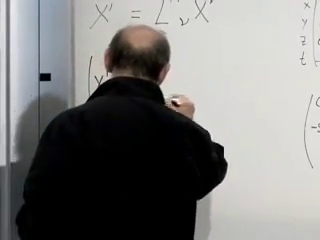
\includegraphics[width=0.8\textwidth]{lecture_06_figure_03.png}\caption{Kontravariante und kovariante Komponenten, die Metrikmatrix und der Beginn der invarianten Kontraktion.}\lectureframe{00:45:00}\end{figure}

Das Senken eines Index ist keine bloße Schreibkonvention. Es berücksichtigt die Vorzeichen, die für die Lorentz-invariante Norm erforderlich sind: \begin{align}
  A_\mu A^\mu
  &=-(A^1)^2-(A^2)^2-(A^3)^2+(A^0)^2,                    \label{eq:l6-norm}\\
  X_\mu X^\mu
  &=t^2-x^2-y^2-z^2.
\end{align} Der zweite Ausdruck ist das invariante Raumzeitintervall vom Ursprung aus. Da \(A^\mu\) sich genauso transformiert wie \(X^\mu\), ist auch ihre Kontraktion invariant.

Die Notation macht zudem eine nützliche Buchführungsregel deutlich: Ein wiederholter Summationsindex tritt einmal oben und einmal unten auf. Zum Beispiel gilt \begin{equation}
  A_\mu A^\mu
  =\eta_{\mu\nu}A^\mu A^\nu.
\end{equation} Die Namen der summierten, sogenannten stummen Indizes können geändert werden, ohne dass sich die Größe ändert.

\begin{classroomqa}
\audiencequestion{Sollte man einen dieser Vektoren als Zeile und den anderen als Spalte auffassen, und spielt ihre Reihenfolge eine Rolle?}
\lecturerresponse{Für die vorliegende Rechnung betrachten wir die indizierten Größen als Komponenten und lassen die Metrik die Kontraktion ausführen; wir brauchen die Diskussion nicht in eine Operatoralgebra mit Zeilen und Spalten umzudeuten. Es handelt sich um gewöhnliche Zahlen, deren Reihenfolge keine Rolle spielt. Bei nichtvertauschenden Operatoren wäre mehr Sorgfalt nötig, doch darum geht es hier nicht.}
\end{classroomqa}

Dieselbe Konstruktion liefert ein inneres Produkt zweier verschiedener Vierervektoren: \begin{equation}
  A\mathbin{\cdot}B=A_\mu B^\mu=A^\mu B_\mu.
\end{equation} Seine Invarianz lässt sich zeigen, ohne eine Lorentz-Matrix explizit hinzuschreiben. Da \(A+B\) und \(A-B\) Vierervektoren sind, sind ihre beiden quadrierten Normen invariant: \begin{align}
  (A+B)^2&=A^2+B^2+2A\mathbin{\cdot}B,\\
  (A-B)^2&=A^2+B^2-2A\mathbin{\cdot}B.
\end{align} Durch Subtraktion erhält man \begin{equation}
  (A+B)^2-(A-B)^2=4A\mathbin{\cdot}B,                    \label{eq:l6-polarization}
\end{equation} und somit ist auch \(A\mathbin{\cdot}B\) invariant. Der Faktor vier ergibt sich unmittelbar aus der Entwicklung.\editorialnote{Das Argument an der Tafel liefert diese Polarisationsidentität; durch die Angabe des Faktors wird die mündlich erläuterte Kürzung eindeutig.}

\begin{figure}[H]\centering
\includegraphics[width=0.8\textwidth]{lecture_06_figure_04.png}\caption{Die beiden invarianten Quadrate, mit denen das innere Produkt verschiedener Vierervektoren isoliert wird.}\lectureframe{00:52:20}\end{figure}

Invariante Größen sind naheliegende Bestandteile physikalischer Gesetze: Anders als eine einzelne Komponente behalten sie ihren Wert beim Wechsel des Bezugssystems bei.

\section{Eigenzeitgeschwindigkeit und Viererimpuls}

Betrachten wir zwei benachbarte Ereignisse auf der Weltlinie eines Teilchens. Ihre Differenz ist der infinitesimale Vierervektor \begin{equation}
  dX^\mu=(dx,dy,dz,dt).
\end{equation} Für eine zeitartige Weltlinie ist die Eigenzeit definiert durch \begin{equation}
  d\tau^2=dX_\mu dX^\mu
  =dt^2-dx^2-dy^2-dz^2.                                  \label{eq:l6-proper-time}
\end{equation} Die Eigenzeitgeschwindigkeit ist \begin{equation}
  U^\mu=\frac{dX^\mu}{d\tau}.                            \label{eq:l6-four-velocity}
\end{equation} Sie beschreibt die Änderungsrate der Raumzeitposition bezüglich der Eigenzeit des Teilchens, nicht bezüglich der Koordinatenzeit eines gewählten Bezugssystems.

Obwohl \(U^\mu\) vier Komponenten hat, sind nur drei davon unabhängig. Teilen wir Gl.~\eqref{eq:l6-proper-time} durch \(d\tau^2\), so erhalten wir \begin{equation}
  U_\mu U^\mu=1.
\end{equation} Damit ist die Vierergeschwindigkeit ein zeitartiger Einheitsvektor. Die Wahl der Zukunftsrichtung legt das Vorzeichen ihrer Zeitkomponente fest.

\begin{classroomqa}
\audiencequestion{Geht die Vierergeschwindigkeit bei Geschwindigkeiten weit unter \(c\) in die gewöhnliche Geschwindigkeit über?}
\lecturerresponse{Ihre drei räumlichen Komponenten nähern sich der gewöhnlichen Geschwindigkeit an, während ihre Zeitkomponente in Einheiten mit \(c=1\) gegen eins geht. Der Zusammenhang folgt, wenn man die Kettenregel anwendet und \(dt/d\tau\) berechnet.}
\end{classroomqa}

Für jede räumliche Komponente gilt \begin{equation}
  U^i=\frac{dx^i}{d\tau}
     =\frac{dx^i}{dt}\frac{dt}{d\tau}
     =v^i\frac{dt}{d\tau}.
\end{equation} Teilen wir Gl.~\eqref{eq:l6-proper-time} durch \(dt^2\), so folgt \begin{equation}
  \left(\frac{d\tau}{dt}\right)^2
  =1-v_x^2-v_y^2-v_z^2
  =1-\boldsymbol v^2.
\end{equation} Also gilt \begin{equation}
  \frac{dt}{d\tau}=\frac{1}{\sqrt{1-\boldsymbol v^2}}
  =\gamma(\lvert\boldsymbol v\rvert),
\end{equation} und \begin{equation}
  U^\mu=(\gamma v_x,\gamma v_y,\gamma v_z,\gamma).
                                                                  \label{eq:l6-u-components}
\end{equation}

\begin{figure}[H]\centering
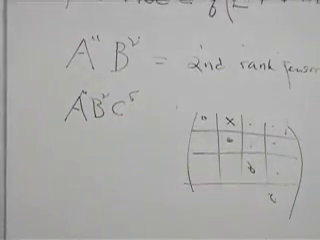
\includegraphics[width=0.8\textwidth]{lecture_06_figure_05.png}\caption{Die Eigenzeitrechnung, aus der \(dt/d\tau=\gamma\) folgt und die die Eigenzeitgeschwindigkeit mit der gewöhnlichen Geschwindigkeit verknüpft.}\lectureframe{01:02:00}\end{figure}

\begin{classroomqa}
\audiencequestion{Bedeutet \(dx^2/dt^2\) eine zweite Ableitung, und entstehen beim Quadrieren eines Vektors nicht gemischte Terme?}
\lecturerresponse{Hier bedeutet es \((dx/dt)^2\), also das Quadrat einer ersten Ableitung. Außerdem steht \(\boldsymbol v^2\) für das euklidische Skalarprodukt \(v_x^2+v_y^2+v_z^2\), nicht für das Quadrat der formalen Summe \(v_x+v_y+v_z\); gemischte Terme treten nicht auf.}
\end{classroomqa}

\begin{classroomqa}
\audiencequestion{Ist das \(v\) in \(\gamma(v)\) die Relativgeschwindigkeit zweier Bezugssysteme oder die Geschwindigkeit des Teilchens?}
\lecturerresponse{Hier ist die Geschwindigkeit des Teilchens im gewählten Bezugssystem gemeint. Die Funktion \(\gamma(v)=1/\sqrt{1-v^2}\) lässt sich für jede Geschwindigkeit auswerten: Bei einem Boost wertet man sie bei der Relativgeschwindigkeit der Bezugssysteme aus, bei der Vierergeschwindigkeit bei der Teilchengeschwindigkeit.}
\end{classroomqa}

Für \(v\ll1\) gilt \(\gamma\simeq1\); die räumlichen Komponenten von \(U^\mu\) nähern sich also \(\boldsymbol v\), und \(U^0\) nähert sich eins. Nähert sich die gewöhnliche Geschwindigkeit der Lichtgeschwindigkeit, so wächst \(\gamma\) und damit wachsen auch alle von null verschiedenen Komponenten der Vierergeschwindigkeit unbegrenzt.

\begin{classroomqa}
\audiencequestion{Müsste \(U^0\) nicht die Einheit einer Geschwindigkeit haben, statt nahe bei der Zahl eins zu liegen?}
\lecturerresponse{Die Einheiten sind weggefallen, weil \(c\) gleich eins gesetzt wurde. Für \(X^0=ct\) gilt \(U^\mu=(\gamma\boldsymbol v,\gamma c)\); die Zeitkomponente nähert sich also \(c\) und \(U_\mu U^\mu=c^2\).}
\end{classroomqa}

Für ein Teilchen mit Ruhemasse \(m\) definieren wir den Viererimpuls durch \begin{equation}
  P^\mu=mU^\mu.
\end{equation} In natürlichen Einheiten gilt \begin{equation}
  P^\mu=(\gamma m\boldsymbol v,\gamma m).
\end{equation} Bei kleinen Geschwindigkeiten nähern sich die ersten drei Komponenten dem Newtonschen Impuls \(m\boldsymbol v\). Setzen wir die Einheiten wieder ein, erhalten wir \begin{equation}
  P^\mu=(\gamma m\boldsymbol v,E/c),
  \qquad E=\gamma mc^2,
\end{equation} und damit \begin{equation}
  E=mc^2+\frac{1}{2}m\boldsymbol v^2+O(mv^4/c^2).
\end{equation} Die Zeitkomponente ist in Einheiten mit \(c=1\) die Energie oder, wenn allen vier Komponenten Impulseinheiten zugewiesen werden, die Energie dividiert durch \(c\).

\begin{classroomqa}
\audiencequestion{Ist die gewöhnliche Geschwindigkeit \(\boldsymbol v\) mit einer angehängten vierten Komponente selbst ein Vierervektor?}
\lecturerresponse{Nein. Die gewöhnliche Dreiergeschwindigkeit transformiert sich nicht wie ein Vierervektor. Der Faktor \(\gamma\) und die Definition über die Eigenzeit sind wesentlich; der Vierervektor ist \(U^\mu\), nicht \(\boldsymbol v\).}
\end{classroomqa}

\section{Warum sich elektrische und magnetische Felder mischen müssen}

Nun machen wir einen kurzen Abstecher von der Relativitätstheorie. Wir beginnen mit der Bewegungsgleichung aus der Zeit vor Einstein und fragen, wie sie umformuliert werden muss, damit sie in jedem Inertialsystem gilt. Die gewöhnliche Beschleunigung ist die Zeitableitung der gewöhnlichen Geschwindigkeit. Ihr vierdimensionales Analogon ist naheliegenderweise \begin{equation}
  A^\mu=\frac{dU^\mu}{d\tau}.
\end{equation} Die räumlichen Komponenten nähern sich bei kleinen Geschwindigkeiten der gewöhnlichen Beschleunigung an. Die vollständige relativistische Bewegungsgleichung stellen wir zurück; zunächst betrachten wir das alte Kraftgesetz.

Für eine Ladung \(q\) in elektrischen und magnetischen Feldern gilt \begin{equation}
  \boldsymbol F=m\boldsymbol a
  =q\left(\boldsymbol E+\boldsymbol v\times\boldsymbol B\right).
                                                                  \label{eq:l6-lorentz-force}
\end{equation} Der elektrische Term hängt nicht von der Teilchengeschwindigkeit ab, der magnetische dagegen schon.

\begin{figure}[H]\centering
\includegraphics[width=0.8\textwidth]{lecture_06_figure_06.png}\caption{Die vorrelativistische Form des Lorentz-Kraftgesetzes, die zur Zusammenfassung von \(\boldsymbol E\) und \(\boldsymbol B\) motiviert.}\lectureframe{01:18:20}\end{figure}

Angenommen, ein Beobachter sieht kein elektrisches Feld, wohl aber ein Magnetfeld und eine bewegte Ladung. Auf die Ladung wirkt eine magnetische Kraft. Im momentanen Ruhesystem der Ladung gilt jedoch \(\boldsymbol v=0\), sodass der magnetische Term in Gl.~\eqref{eq:l6-lorentz-force} verschwindet. Die physikalische Weltlinie wird nicht dadurch inertial, dass sich die Koordinaten ändern; die Kraft im neuen Bezugssystem muss daher einen elektrischen Beitrag enthalten. Genauer gesagt lässt sich eine von null verschiedene Viererbeschleunigung durch einen Wechsel des Inertialsystems nicht in null überführen, auch wenn die Dreierbeschleunigung und ihre Komponenten transformiert werden.\editorialnote{Diese Aussage über die Viererbeschleunigung ist die invariante Form des Arguments aus der Vorlesung und vermeidet es, die gewöhnliche Dreierbeschleunigung selbst als bezugssysteminvariant zu behandeln.}

Elektrische und magnetische Felder müssen sich folglich ineinander transformieren. Zusammen haben sie sechs Komponenten und bilden daher weder einen einzelnen Skalar noch einen Vierervektor. Wir benötigen ein neues Transformationsobjekt.

\section{Tensoren: eine Transformation für jeden Index}

Ein Skalar lässt sich als Tensor nullter Stufe bezeichnen; er hat keine Indizes. Ein Vierervektor ist ein Tensor erster Stufe mit einem Index, der vier mögliche Werte annimmt. Das einfachste Beispiel für einen Tensor zweiter Stufe ist ein Produkt \begin{equation}
  A^\mu B^\nu.
\end{equation} Jeder Index kann vier Werte annehmen; das Objekt hat also \(4^2=16\) Komponenten und lässt sich als Array der Größe \(4\times4\) darstellen. Das Produkt dreier Vektoren \begin{equation}
  A^\mu B^\nu C^\sigma,
\end{equation} hat \(4^3=64\) Komponenten und ist ein Tensor dritter Stufe. Bei höheren Stufen setzt sich das Muster fort. Wichtiger als der Name ist die Regel, die das Objekt definiert.

Wenn \begin{equation}
  A'^{\mu}=\Lambda^\mu{}_{\nu}A^\nu,
  \qquad
  B'^{\sigma}=\Lambda^\sigma{}_{\tau}B^\tau,
\end{equation} gilt, transformiert sich ihr Produkt gemäß \begin{equation}
  A'^{\mu}B'^{\sigma}
  =\Lambda^\mu{}_{\nu}\Lambda^\sigma{}_{\tau}
   A^\nu B^\tau.
\end{equation} Daraus ergibt sich das definierende Transformationsgesetz für einen kontravarianten Tensor zweiter Stufe: \begin{equation}
  T'^{\mu\sigma}
  =\Lambda^\mu{}_{\nu}\Lambda^\sigma{}_{\tau}T^{\nu\tau}.
                                                                  \label{eq:l6-tensor-transform}
\end{equation} Für jeden Index gibt es eine Lorentz-Matrix. Über die wiederholten Indizes \(\nu\) und \(\tau\) wird summiert; die freien Indizes \(\mu\) und \(\sigma\) bezeichnen die im gestrichenen Bezugssystem berechnete Komponente.

\begin{figure}[H]\centering
\includegraphics[width=0.82\textwidth]{lecture_06_figure_07.png}\caption{Die Transformation zweier Vektoren und das daraus folgende Transformationsgesetz mit zwei Matrizen für einen Tensor zweiter Stufe.}\lectureframe{01:27:15}\end{figure}

Ein Tensor muss nicht das Produkt einzelner Vektoren sein. Sowohl \(A^\mu B^\nu\) als auch \(A^\nu B^\mu\) gehorchen dem Tensor-Transformationsgesetz, ebenso ihre Summe und jede Summe der Form \begin{equation}
  A^\mu B^\nu+C^\mu D^\nu.
\end{equation} Die Definition ist das Transformationsgesetz, nicht eine bestimmte Produktdarstellung. Ein Tensor dritter Stufe erhält eine dritte Lorentz-Matrix und so weiter.

\section{Symmetrische und antisymmetrische Tensoren}

Zwei Klassen von Tensoren zweiter Stufe werden besonders nützlich sein. Ein symmetrischer Tensor erfüllt \begin{equation}
  T^{\mu\nu}=T^{\nu\mu},
\end{equation}, sodass spiegelbildlich zur Diagonalen liegende Einträge übereinstimmen. Seine vier Diagonaleinträge und die sechs Einträge auf einer Seite der Diagonalen bestimmen alle übrigen. Damit hat er \begin{equation}
  4+6=10
\end{equation} unabhängige Komponenten.

Ein antisymmetrischer Tensor erfüllt \begin{equation}
  T^{\mu\nu}=-T^{\nu\mu}.                                \label{eq:l6-antisymmetry}
\end{equation} Setzen wir \(\mu=\nu\) in Gl.~\eqref{eq:l6-antisymmetry} ein, erhalten wir \(T^{\mu\mu}=-T^{\mu\mu}\); daher verschwinden alle Diagonaleinträge. Die sechs Einträge in einer Dreieckshälfte bestimmen die anderen sechs mit umgekehrtem Vorzeichen. Es gibt somit genau sechs unabhängige Komponenten.

\begin{figure}[H]\centering
\includegraphics[width=0.82\textwidth]{lecture_06_figure_08.png}\caption{Ein ausgefülltes antisymmetrisches Array der Größe \(4\times4\): Nullen auf der Diagonalen und entgegengesetzte Vorzeichen auf beiden Seiten.}\lectureframe{01:34:25}\end{figure}

Diese Anzahl ist der entscheidende Hinweis. Die drei elektrischen und die drei magnetischen Komponenten lassen sich in einem einzigen antisymmetrischen Tensor zweiter Stufe zusammenfassen.

\section{Der elektromagnetische Feldstärketensor}

Wir ordnen die Raumzeitindizes in Zeilen und Spalten der Reihenfolge \((1,2,3,0)=(x,y,z,t)\) entsprechend an. Die Darstellung an der Tafel lautet \begin{equation}
  F_{\mu\nu}=
  \begin{pmatrix}
    0    & -B_3 & B_2  & E_1\\
    B_3  & 0    & -B_1 & E_2\\
    -B_2 & B_1  & 0    & E_3\\
    -E_1 & -E_2 & -E_3 & 0
  \end{pmatrix}.                                         \label{eq:l6-field-tensor}
\end{equation} Die rein räumlichen Komponenten enthalten das Magnetfeld; die Komponenten mit einem räumlichen und einem Zeitindex enthalten das elektrische Feld. Wegen der Antisymmetrie ergeben sich die Einträge unterhalb der Diagonalen aus den Einträgen oberhalb der Diagonalen.

\begin{classroomqa}
\audiencequestion{Sind die magnetischen Einträge alle negativ, und entsprechen die Indizes \(x,y,z\)?}
\lecturerresponse{Die Vorzeichen im oberen räumlichen Dreieck wechseln wie dargestellt: \(-B_3,+B_2,-B_1\) Die Indizes \(1,2,3\) entsprechen \(x,y,z\), während \(0\) die Zeit bezeichnet. Die Spiegelung an der Diagonalen kehrt jedes Vorzeichen um.}
\end{classroomqa}

\begin{figure}[H]\centering
\includegraphics[width=0.82\textwidth]{lecture_06_figure_09.png}\caption{Der vollständige elektromagnetische Feldstärketensor in der Vorlesung verwendeten Anordnung mit den räumlichen Komponenten zuerst.}\lectureframe{01:41:05}\end{figure}

Üblicherweise schreibt man \(F_{\mu\nu}\) statt eines allgemeinen \(T_{\mu\nu}\). Der Dozent vermutet, der Buchstabe könne auf Faraday verweisen, sagt aber ausdrücklich, dass ihm die Geschichte dieser Notation nicht bekannt ist. Entscheidend sind hier die Antisymmetrie und die sechs Feldkomponenten, nicht diese Vermutung über den Buchstaben.

\begin{classroomqa}
\audiencequestion{Stellt jeder Matrixeintrag die Stärke eines Feldes in der angegebenen Koordinatenebene dar?}
\lecturerresponse{Er ist eine Komponente des elektromagnetischen Feldstärketensors. Die Einträge mit einem Zeitindex sind elektrische Komponenten, die räum--räumlichen Einträge codieren magnetische Komponenten.}
\end{classroomqa}

Klammern wir die Zeile und die Spalte mit dem Zeitindex aus. Der verbleibende antisymmetrische \(3\times3\)-Block ist magnetisch. Seine unabhängigen Komponenten kann man sich zyklisch merken: \begin{equation}
  F_{12}=-B_3,
  \qquad F_{23}=-B_1,
  \qquad F_{31}=-B_2.                                   \label{eq:l6-magnetic-cycle}
\end{equation} Geht man von der ersten Beziehung aus, rückt man die Indizes der Reihe nach entlang \(1\to2\to3\to1\) weiter. Äquivalent dazu gilt \begin{equation}
  F_{ij}=-\epsilon_{ijk}B_k,
\end{equation} mit \(\epsilon_{123}=+1\).\editorialnote{Die Levi--Civita-Formel ist die kompakte Standardform der an der Tafel Schritt für Schritt entwickelten zyklischen Regel.}

\begin{figure}[H]\centering
\includegraphics[width=0.82\textwidth]{lecture_06_figure_10.png}\caption{Die zyklischen räumlichen Komponenten, die das Magnetfeld im antisymmetrischen Tensor codieren.}\lectureframe{01:46:20}\end{figure}

Die Zuordnungen für das elektrische Feld sind direkter: \begin{equation}
  E_1=F_{10},
  \qquad E_2=F_{20},
  \qquad E_3=F_{30}.
\end{equation}

Das Magnetfeld hat folglich zwei nützliche Darstellungen. Im dreidimensionalen Raum lässt sich ein axialer Vektor mit drei Komponenten einem antisymmetrischen \(3\times3\)-Tensor zuordnen. In der Raumzeit ist es dagegen nur der räumliche Anteil des sechskomponentigen Tensors \(F_{\mu\nu}\). Diese Zuordnung ist spezifisch für drei Dimensionen: Ein antisymmetrischer \(4\times4\)-Tensor hat sechs unabhängige Komponenten und lässt sich nicht mit einem Vierervektor identifizieren.\editorialnote{Unter eigentlichen Drehungen verhält sich das Magnetfeld wie ein Vektor; unter Spiegelungen ist es genauer gesagt ein Axialvektor oder Pseudovektor.}

Der Zweck dieser Konstruktion ist nicht, um des Zählens willen Komponenten zu zählen. Da \(F_{\mu\nu}\) sich als Tensor transformiert, mischt ein Lorentz-Boost seine elektrischen und magnetischen Komponenten automatisch. In der nächsten Vorlesung lässt es sich mit Vierergeschwindigkeit und Viererbeschleunigung kombinieren, um Gl.~\eqref{eq:l6-lorentz-force} durch eine kovariante Bewegungsgleichung zu ersetzen.

\section{Fragen zu Einstein und Minkowski}

In den letzten Minuten geht es nicht mehr um den Formalismus, sondern um seine historische Entstehung. Die Antworten werden als Erinnerungen und nicht als gesicherte Geschichtsdarstellung gegeben; diese Einschränkung gehört zum Gespräch.

\begin{classroomqa}
\audiencequestion{Suchte Einstein aus konzeptionellen Gründen nach einer Lorentz-invarianten Formulierung, oder trieben ihn bestimmte Beobachtungen dazu?}
\lecturerresponse{Der Grundsatz, dass die Naturgesetze in jedem Inertialsystem dieselbe Form haben sollten, war für seine Überlegungen zentral. Zudem gab es experimentelle Hinweise zum Licht und dazu, dass sich eine Bewegung durch einen Äther nicht nachweisen ließ. Der Dozent ist sich jedoch ausdrücklich nicht sicher, welche Ergebnisse Einstein kannte oder wie stark sie ihn beeinflussten. Der konzeptionelle Druck bestand darin, dass Maxwells Gleichungen und die Lorentz-Kraft dem Relativitätsprinzip gehorchen sollten. Dafür müssen sich elektrische Felder, magnetische Felder und Geschwindigkeitskomponenten gemeinsam transformieren.}
\end{classroomqa}

Einsteins Darstellung von 1905 verwendete nicht die hier benutzte kompakte Vierervektorschreibweise. Sie ging komponentenweise vor und schrieb die nötigen Faktoren von \(\gamma\) und der Geschwindigkeit ausdrücklich hin. Minkowski ordnete dieselbe Struktur später geometrisch als vierdimensionale Raumzeit.

\begin{classroomqa}
\audiencequestion{Sträubte sich Einstein gegen Minkowskis Raumzeitformulierung, und wie bald führte Minkowski sie ein?}
\lecturerresponse{Die in der Vorlesung wiedergegebene Erinnerung lautet, dass Einstein die vierdimensionale geometrische Sprache anfangs nicht begrüßte, ihren Nutzen aber bald erkannte. Als Zeitpunkt werden vorsichtig ungefähr zwei Jahre nach der Arbeit von 1905, vielleicht 1907, genannt; der Sprecher betont, dass er sich erinnert und die historische Einordnung nicht gesichert darstellt.}
\end{classroomqa}

\begin{classroomqa}
\audiencequestion{War Minkowski Mathematiker oder Physiker, wozu hat er sonst noch beigetragen, und wurde er von Lorentz oder FitzGerald beeinflusst?}
\lecturerresponse{Eine sichere Antwort wird nicht beansprucht. Die Unterscheidung zwischen Mathematiker und Physiker wurde nicht weiterverfolgt, eine Korrektur aus dem Publikum unterbricht eine allgemeine Bemerkung zu Minkowskis weiteren Arbeiten, und mögliche Einflüsse bleiben ausdrücklich ungewiss. Der gesicherte Punkt für diese Diskussion ist Minkowskis entscheidende geometrische Formulierung der Relativitätstheorie in vierdimensionaler Notation.}
\end{classroomqa}

\begin{classroomqa}
\audiencequestion{Gab es die Transformationen, die \(\boldsymbol E\) und \(\boldsymbol B\) mischen, schon in Einsteins Arbeit von 1905?}
\lecturerresponse{Ja, aber sie waren komponentenweise und nicht in Form einer einzigen Feldtensor-Gleichung geschrieben. Der Vergleich in der Vorlesung gilt den Komponentengleichungen von Maxwell: Der Inhalt kann bereits vorhanden sein, bevor eine kompakte Notation seine gemeinsame Struktur sichtbar macht. Minkowskis Beitrag bestand darin, diese Struktur in der Sprache der Raumzeit systematisch darzustellen.}
\end{classroomqa}

Damit kehren wir zu dem mathematischen Punkt zurück, mit dem wir begonnen haben. Komponenten sind für Berechnungen unverzichtbar, doch das Gesetz wird verständlich, wenn man sie als Bestandteile eines einzigen Objekts erkennt, das sich transformiert. Als Nächstes gilt es, mithilfe von \(F_{\mu\nu}\) die Bewegungsgleichung des geladenen Teilchens so zu formulieren, dass sie in allen Inertialsystemen dieselbe Form hat.